\documentclass[review]{elsarticle}

\usepackage[colorlinks]{hyperref}
\usepackage[colorinlistoftodos]{todonotes}
\usepackage{verbatim}
\usepackage[utf8]{inputenc}
\usepackage[T1]{fontenc}
\usepackage{adjustbox}
\usepackage{multirow}
\usepackage{longtable}
\usepackage{booktabs}
\usepackage{lineno,hyperref}
\modulolinenumbers[5]

\journal{BTAS}

%%%%%%%%%%%%%%%%%%%%%%%
%% Elsevier bibliography styles
%%%%%%%%%%%%%%%%%%%%%%%
%% To change the style, put a % in front of the second line of the current style and
%% remove the % from the second line of the style you would like to use.
%%%%%%%%%%%%%%%%%%%%%%%

%% Numbered
%\bibliographystyle{model1-num-names}

%% Numbered without titles
%\bibliographystyle{model1a-num-names}

%% Harvard 
%\bibliographystyle{model2-names.bst}\biboptions{authoryear}

%% Vancouver numbered
%\usepackage{numcompress}\bibliographystyle{model3-num-names}

%% Vancouver name/year
%\usepackage{numcompress}\bibliographystyle{model4-names}\biboptions{authoryear}

%% APA style
\bibliographystyle{model5-names}\biboptions{authoryear}

%% AMA style
%\usepackage{numcompress}\bibliographystyle{model6-num-names}

%% `Elsevier LaTeX' style
%\bibliographystyle{elsarticle-num}
%%%%%%%%%%%%%%%%%%%%%%%

\begin{document}

\begin{frontmatter}

\title{Reverse Engineering a Bronze Cannon from the\\La Belle Shipwreck}

%% Group authors per affiliation:
\author{Robert Z. Selden, Jr.\textsuperscript{a,b}* and Bradford M. Jones\textsuperscript{c}}
\address[1]{Heritage Research Center, Stephen F. Austin State University, USA}
\address[2]{Cultural Heritage Department, Jean Monnet University, FR}
\address[3]{Archeology Division, Texas Historical Commission, Austin, USA}
\cortext[cor1]{Corresponding author, Robert Z. Selden Jr. (zselden@sfasu.edu)}

\begin{abstract}
%% Text of abstract 
The goal of this project was to scan and reverse engineer one of three bronze cannons (41MG86 - 11900-1) recovered from the La Belle excavation, and currently on exhibit at the Bullock Texas State History Museum in Austin, Texas. A freeform computer aided design (CAD) model was generated based upon the topology of the 3D mesh in Geomagic Design X with a desired maximum deviation of 0.1 mm between the model and the mesh. Deviations were calculated in Geomagic Control X using the surface model as the reference data, and the mesh as the measured data. A custom patch network was subsequently designed using a series of iterative revisions until the whole of the surface model met with the specified tolerance. The 3D surface model of the cannon will be replicated in a variety of media at variable scales for use in exhibits and for educational and promotional material for the Texas Historical Commission, the Republic of France, and their partner museums.
\end{abstract}

\begin{keyword}
France \sep shipwreck \sep nautical archaeology \sep La Belle \sep cannon
%% keywords here, in the form: keyword \sep keyword

%% MSC codes here, in the form: \MSC code \sep code
%% or \MSC[2008] code \sep code (2000 is the default)

\end{keyword}

\end{frontmatter}

\linenumbers

\section*{Background}

Three bronze cannons raised from the hull of French explorer Rene Cavalier La Sieur de La Salle's lost ship La Belle in Matagorda Bay, Texas, are among the most celebrated and iconic of the nearly two million artefacts excavated from the CE 1686 wreck site by the Texas Historical Commission (THC) \citep{RN5767}. The first was raised in the summer of 1995 after testing a magnetic anomaly detected by State Marine Archeologist J. Barto Arnold in the vicinity of La Belle's last recorded location, where the remains of a 17\textsuperscript{th} or 18\textsuperscript{th} century wooden-hulled vessel \citep{RN5766,RN5765} was found. It was recognised that the cannon might aid in the identification of the wreck, and it was sent to Dr. Donald H. Keith at the Ships of Discovery Conservation Laboratory at the Corpus Christi Museum of Science and History for cleaning and conservation.

Cleaning and conservation revealed an ornately decorated bronze (four-pound) cannon likely corresponding to one of the four granted to La Salle by the King for field artillery \citep{RN5763,RN5764}. Stylised acanthus leaves decorate the base, mid-section, and muzzle of each, and the lifting handles atop the cannon are fashioned as toothy dolphins. A stylised monogram of French King Louis XIV is prominently displayed on the breech below, where a series of inscriptions on the base ring of the cannon read \textit{N\textsuperscript{o} 4} and \textit{no  741}. The chase of the barrel bears the armorial device of Louis Alexandre de Bourbon, le Comte de Vermandois, the third child from Louis XIV's affair with the Duchess of Valiere, who in CE 1669 was appointed the Grand Admiral of France at the age of 2, and served until his death in CE 1683 \citep[354]{RN5763}. During this period, the bronze cannons produced in royal foundries displayed a version of his armorial device, a practice that aided in refining the period during the reign of Louis XIV when the cannon was cast. This predates La Salle's expedition, which set sail in the summer of CE 1684, and the presence of the cannon aided in verifying that the shipwreck was indeed the La Belle.

In 1997-1998 the remainder of the vessel was excavated by the THC under the direction of Dr. James E. Bruseth. In the course of that excavation, two additional bronze cannons--nearly identical to the first--were uncovered in the bottom of the hull (Figure ~\ref{fig:FigExcavate}) \citep{RN5763,RN5762,RN5761}. The cannon selected for 3D scanning, and described herein, was one of two that were recovered \textit{in-situ}, found atop the ballast and beneath the cargo of the main hold. A fourth cannon was identified as having been a part of the La Belle cargo; however, it was previously removed by an unknown party, leaving behind only the impression of the cannon on the sea floor \citep{RN5763}.

\begin{figure}[ht]\centering
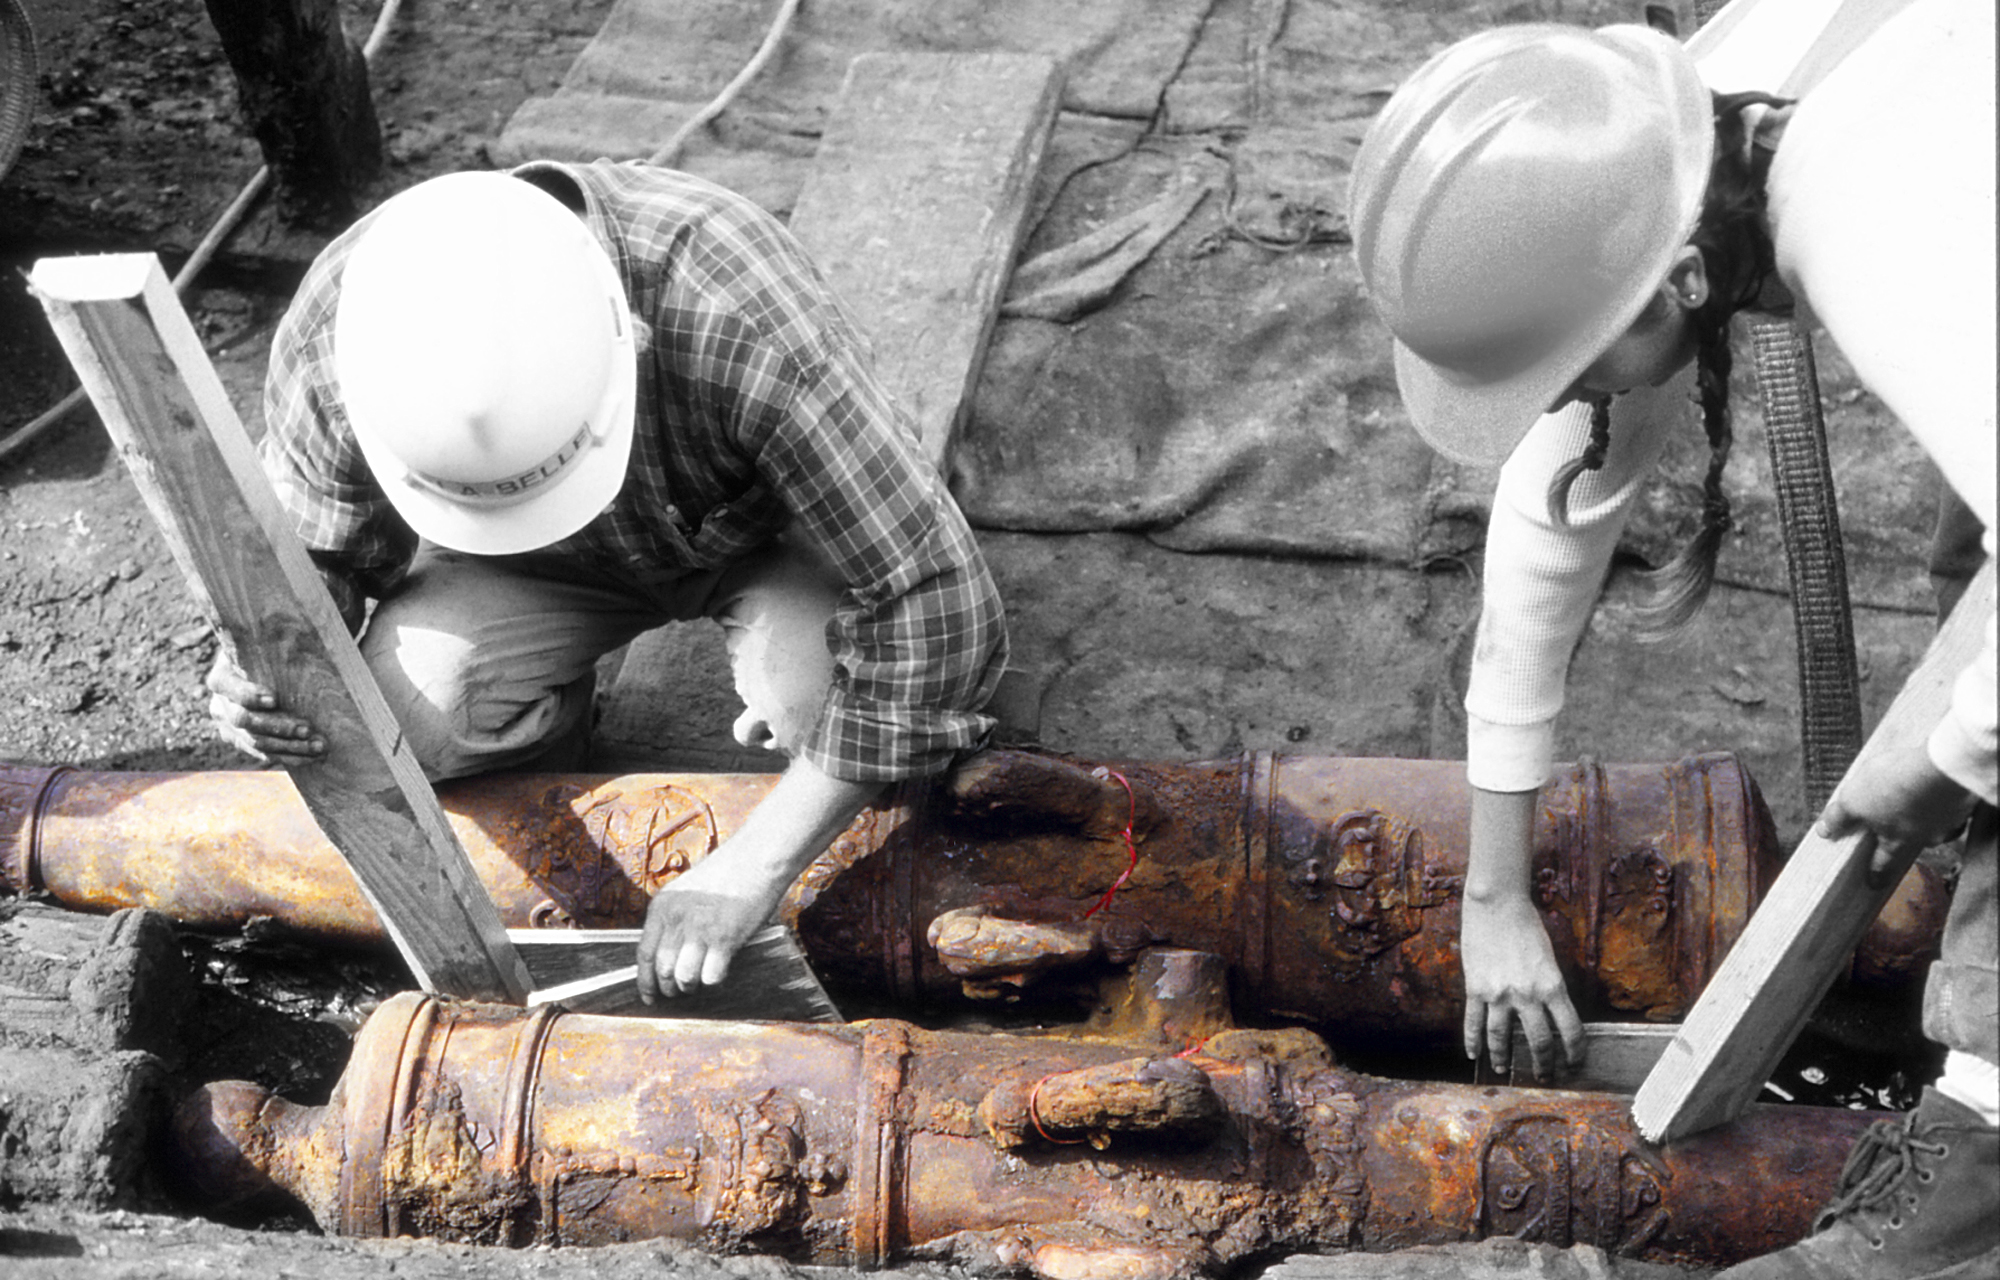
\includegraphics[width=\linewidth]{FigExcavate2}
\caption{Image of cannons 84 (41MG86 - 11900-1 - back) and 85 (41MG86 - 11350 - front) being excavated from the hull of La Belle during the THC excavations.}
\label{fig:FigExcavate}
\end{figure}

The two cannons recovered \textit{in-situ} were transported to the Conservation Research Laboratory at Texas A\&M University, then to Keith for analyses (Figure ~\ref{fig:FigConserve}). Both were found to bear decorations nearly identical to the first, with minor variations typical of replicated moulds based upon the master \citep[361]{RN5763}. Like the first cannon, which bore the inscription \textit{N\textsuperscript{o} 4 no 741}, these two were marked in the same location on the base ring with \textit{746 \# N\textsuperscript{o} 84} and \textit{744 \# N\textsuperscript{o} 85}, respectively (Figure ~\ref{fig:FigBASE}).

\begin{figure}[ht]\centering
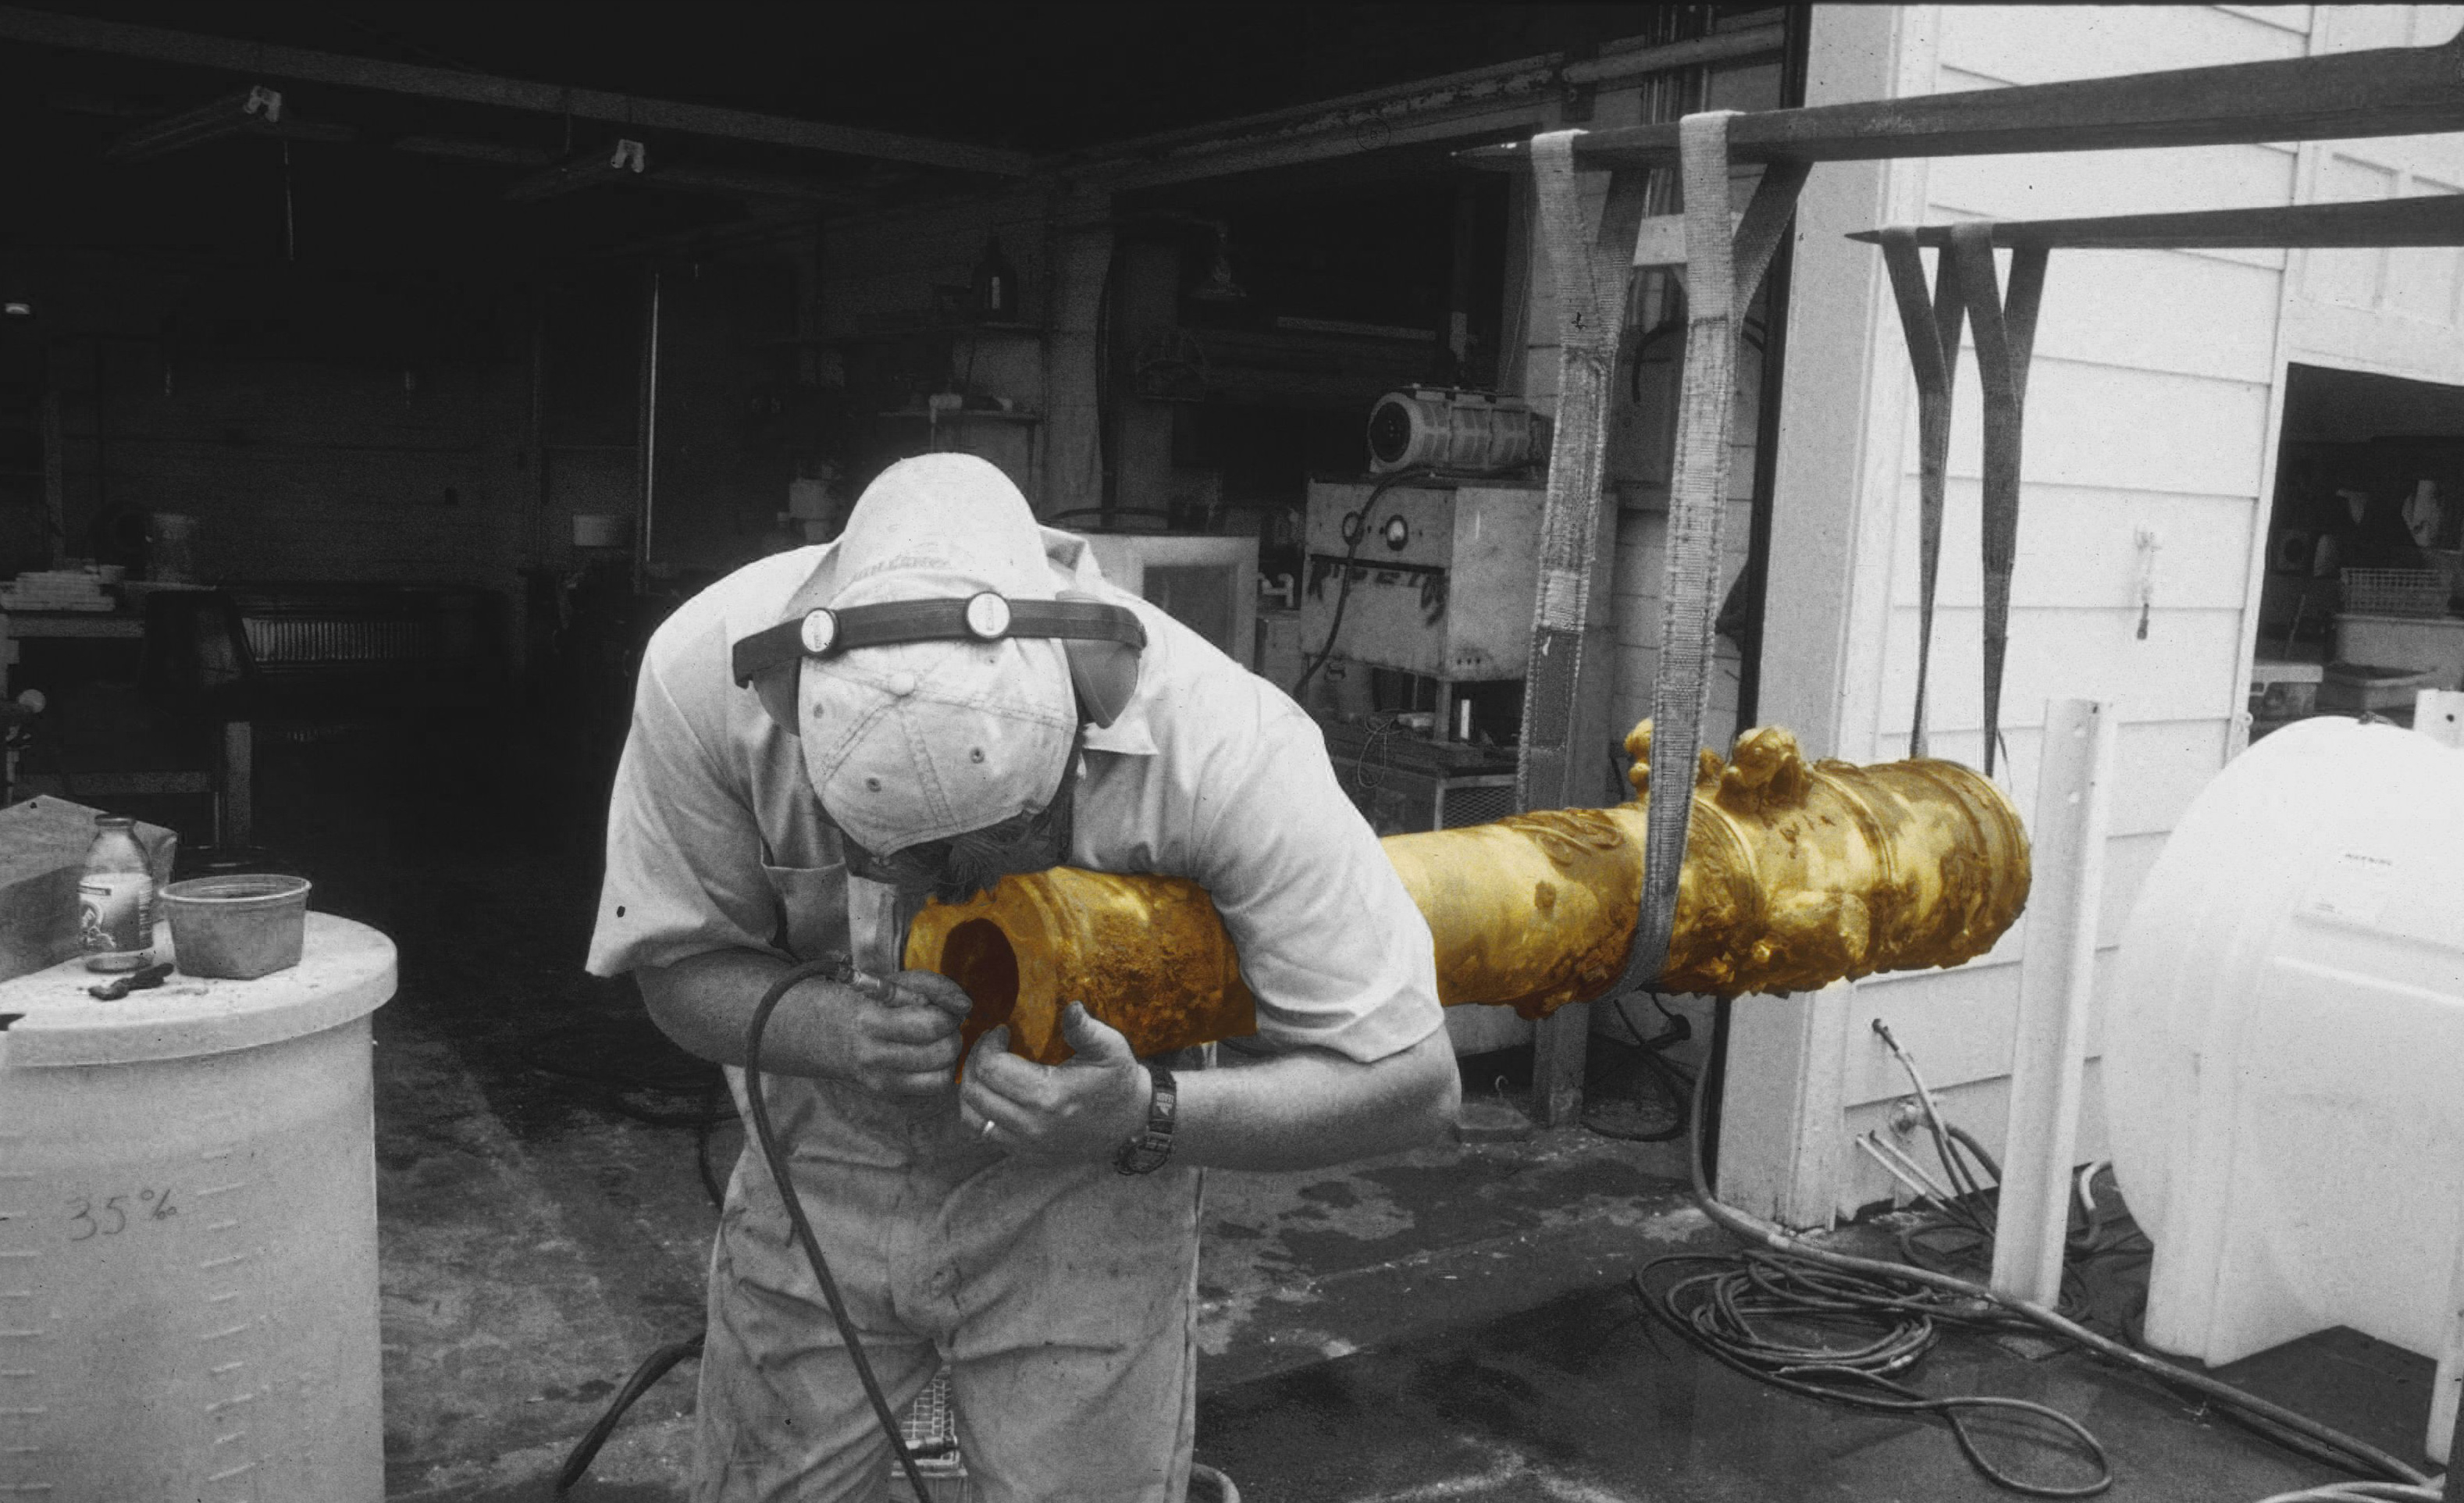
\includegraphics[width=\linewidth]{FigConserve2}
\caption{Image of Cannon No. 84 (41MG86 - 11900-1) undergoing conservation.}
\label{fig:FigConserve}
\end{figure}

\begin{figure}[ht]\centering
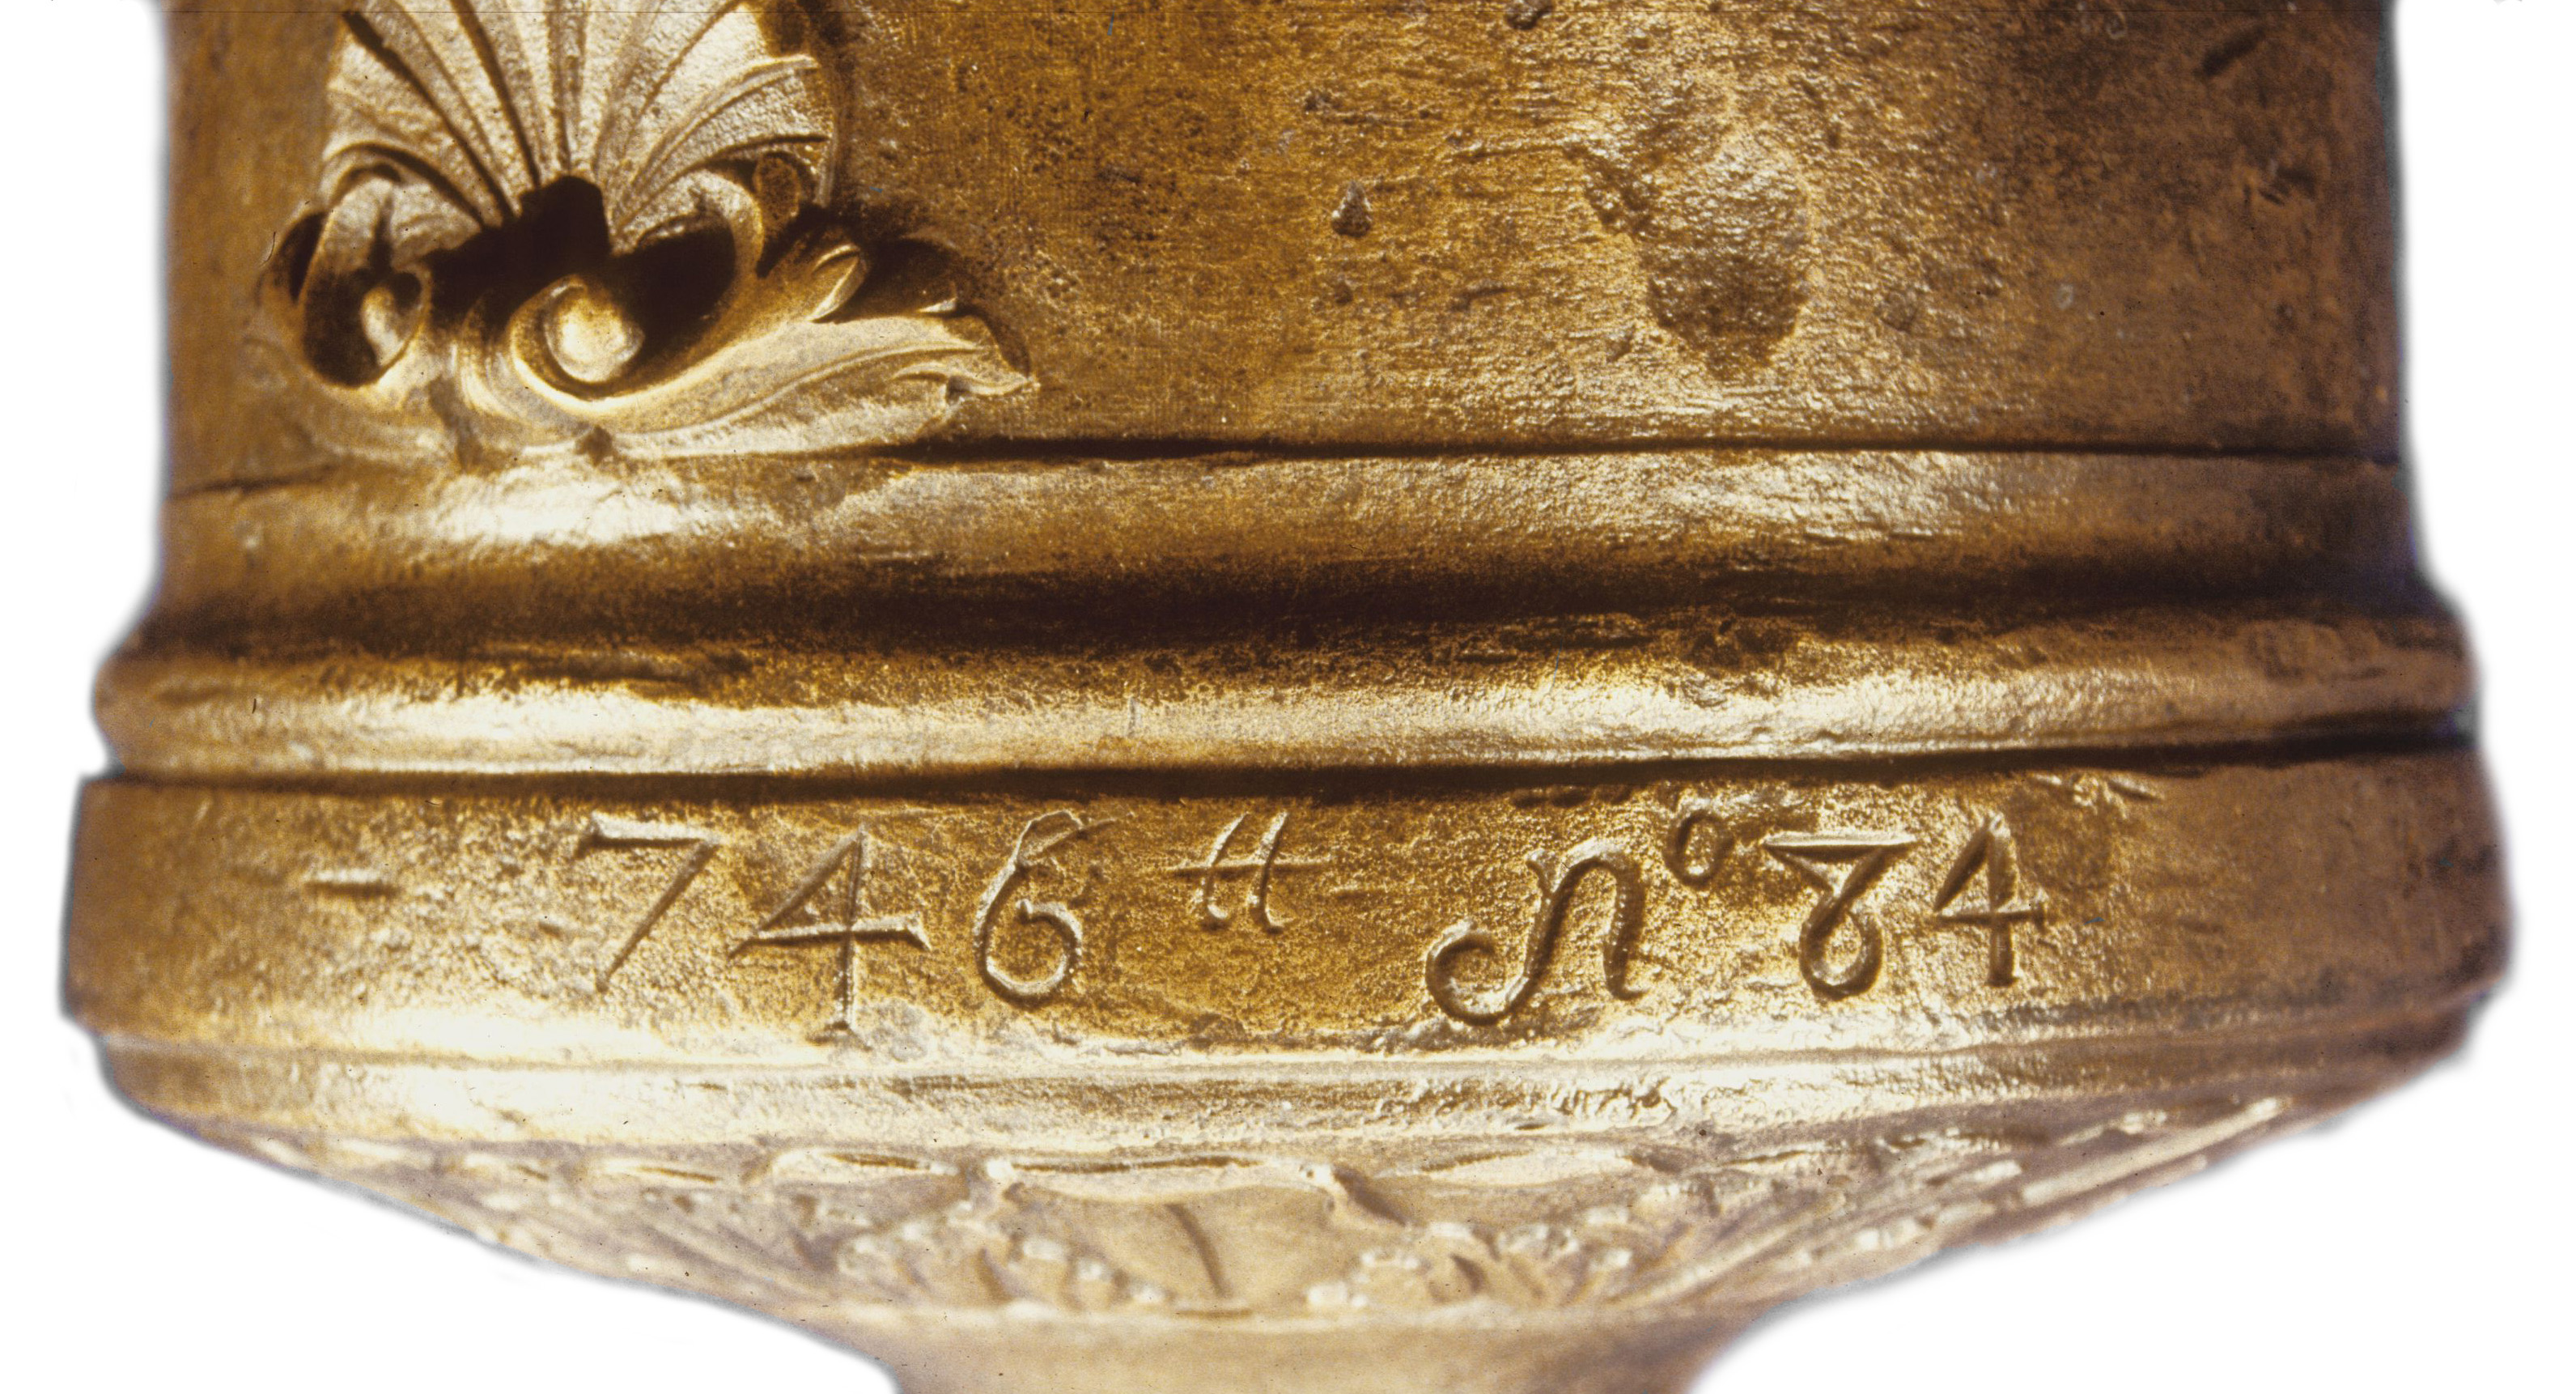
\includegraphics[width=\linewidth]{FigBASE2}
\caption{Close up of the markings on the base of 41MG86 - 11900-1.}
\label{fig:FigBASE}
\end{figure}

Manufacturing details for the cannons were revealed through a combination of archival research and detailed studies of the cannon by Keith and colleagues \citep[359-367]{RN5763}. The lack of visible mould lines on the cannon aligns with historical accounts of French bronze casting techniques, where a one-time ceramic mould was suspended vertically with the muzzle of the cannon pointed upward, and a reservoir for the molten metal mounted to the top. The mould for each cannon was generated using a pattern, and constructed around a wooden core wrapped in rope to create the desired wall thickness. Each mould was then finished in clay onto which trunnions, cascabels, lifting handles and other decorative elements were added using a series of secondary moulds that ensured general uniformity of the overall design. However, the distinctive attributes of individual moulds means that each cannon displays minor variations on the common theme. This can be seen in the variable sharpness of the armorial device, and the placement of floral patterns, which differ between the three cannons. Contrasting textures and proportions along the surface of the cannons indicate the fluctuating conditions associated with each pour, and the distinctive surface textures noted around the ornamentation are believed to be associated with the application of secondary moulds; however, additional research is necessary to understand the exact process through which those textures where rendered.

In addition to the mould, a core was used to create the bore as the metal was added, which was stabilised by iron armatures fixed inside the barrel, near the bottom and top of the cannon. An unexpected outcome of the initial analysis was the discovery of spiral grooves inside the bore, which appear to be remnants associated with the wire wrapping of the original core, which was preserved through the manufacturing process. Keith proposes the presence of the grooves may indicate that both bores were only lightly reamed after manufacture, or that the cannons had seen little use, and he notes the need to more carefully consider bore attributes in understanding the manufacturing process as it relates to cannons from this period \citep[366]{RN5763}.

More detailed information associated with the manufacture of the individual cannons was revealed by the unique base ring inscriptions. Though initially unclear in their significance, archival research in France by John de Bry identified a CE 1682 inventory of the armaments of the ship Le Faucon, listing three bronze four-pound cannons with identical inventory numbers and weights to those recovered from the La Belle, as well as the record of fourth, which is likely to correspond with the cannon missing from the hull. Records also indicate that the cannons were cast by Jean La Tache, the master founder of the arsenal of Rochefort, from CE 1670-1679 \citep[356-357]{RN5763}. Le Faucon was constructed in Rochefort between CE 1673-74 and La Tache likely cast the bronze cannons for use aboard the ship at that time. Though cast to serve a naval function, by the time  the bronze cannons were placed in the hull of La Belle, their use was prescribed for terrestrial applications to guard a second settlement or conduct military campaigns.

\section*{Reverse Engineering}

Reverse engineering can be conceived of as a form of mechanical dissection or backward problem solving \citep{RN5750}, and summarised as a process of reasoning in reverse from a technological artefact to the problem that it was created to address \citep{RN5751}. Theories associated with reverse engineering are not widely applied in archaeology \citep{RN5752}; however, there are a number of archaeological examples associated with finite elements analysis (FEA) that do point toward a broader interest in the application of reverse engineering principles. Examples of FEA in archaeological practice can be seen in analyses of ceramics \citep{RN327,RN5753}, the USS Arizona \citep{RN325}, the Albolafia waterwheel \citep{RN5754}, and ancient architecture \citep{RN5755}.

Reverse engineering is largely an exploratory enterprise with the purpose of understanding design and---where possible---the method of manufacture in cases where written records are not available. Historic and archaeological applications that employ reverse engineering practices include ceramics \citep{RN5769,RN5770} headstones \citep{RN456}, inscriptions \citep{RN5756}, a Greek Lyre \citep{RN5757}, historic structures and monuments \citep{RN5771,RN5772}, general digital restoration \citep{RN5760}, a foot rest bracket for a historic bicycle \citep{RN5758}, and an assessment of the reverse engineering process for cultural heritage conservation \citep{RN5759}. Reverse engineering of the cannon follows in-step with the studies mentioned above, but differs in that it enlists a 3D scan-to-CAD workflow where the surface model is iteratively refined to meet the specific tolerances specified by project parameters through pairing CAD with computer aided inspection, thus accurately integrating the many blemishes and imperfections incurred during historic trans-Atlantic transport and use.

\section*{Purpose}

The impetus for designing a surface model of the cannon emerged from discussions between the THC, the Bullock Texas State History Museum, and the French Musée national de la Marine concerning a future exhibit in France that will present La Salle's expedition through the archaeology of the ship. As a critical piece of the discovery, excavation and identification of the La Belle, the public display of one of the ornately decorated bronze cannons was considered essential. However, the transatlantic shipment of a historic bronze cannon that weighs over 700 pounds raised a number of logistical and financial concerns.

While the construction of a mould from the original was immediately considered an option, it became apparent that 3D scanning and modeling was not only a less invasive method, but could efficiently create the type of easily transferable model needed to provide French exhibit designers with the opportunity to replicate the cannon in a variety of media. Scanning the cannon had the added benefit of a creating a digital record that can be employed in educational and promotional material for the THC, the Republic of France, and other partner museums, while simultaneously providing for the continued study of this important artefact. While the French exhibition has been delayed due to renovations, the THC proceeded with the project in 2016 in order to take advantage of the additional research and public outreach opportunities that the project could generate.

\section*{Project Workflow and Methods}

The project-specific workflow designed to model the cannon included the requirement that the deviation from the mesh should be no greater than 0.1 mm is outlined in Figure \ref{fig:FigWorkflow}. The process began by generating the 3D scan data, which was subsequently processed in VXelements and Geomagic Design X. Following the initial design of the freeform surface model, computer aided inspection software (Geomagic Control X) was used to ensure that the model met with the specific design parameters of the project. Should an area of the surface model be found to exceed the 0.1 mm tolerance, those areas were noted, re-modeled, inspected, then refined prior to a subsequent inspection. This iterative process of model-inspect-refine continued until the whole of the surface model met with the tolerance required by the project. The final freeform CAD model was exported to KeyShot for visualisation, and to SolidWorks where additional components (i.e., carriage, etc.) can be added and integrated with the model of the cannon, or digitally placed within the reconstructed CAD model of the vessel itself.

\begin{figure}[ht]\centering
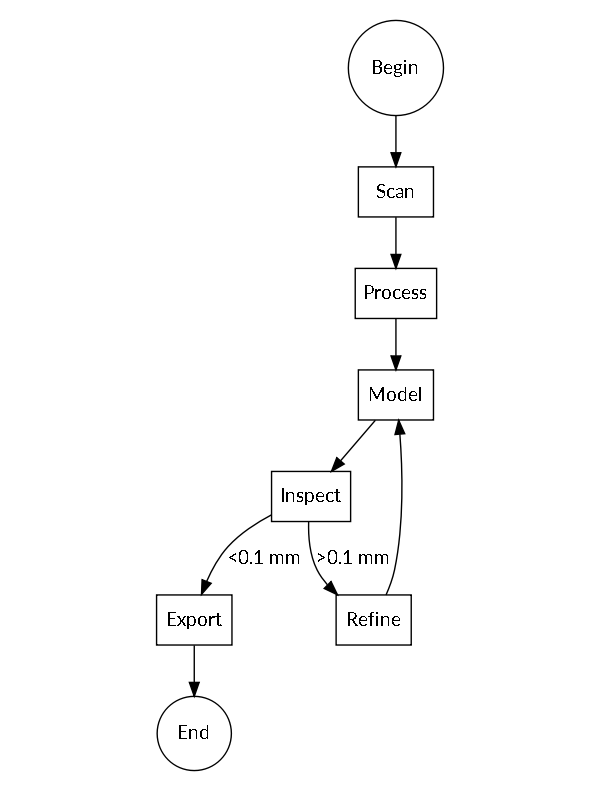
\includegraphics[width=0.6\linewidth]{FigWorkflow}
\caption{Workflow designed to reverse engineer the cannon recovered from the La Belle shipwreck.}
\label{fig:FigWorkflow}
\end{figure}

The cannon (41MG86 - 11900-1) was scanned with a Creaform GoSCAN20 running VXElements via the scanner direct control function in Geomagic Design X. Scan data were collected at 0.3 mm, then refined to 0.1mm in post. The point cloud associated with the unprocessed scan data was saved and exported prior to post-processing. Scan data were subsequently imported to Geomagic Design X, where the final mesh was aligned and processed. Post-processing of the 3D mesh began by correcting issues with non-manifold poly-vertices, folded poly-faces, dangling poly-faces, small clusters, small poly-faces, non-manifold poly-faces, crossing poly-faces, and small tunnels in the 3D mesh. Due to the limitations of 3D scanning, those sections of the mesh associated with the vent and the bore of the cannon were cut, and the mesh boundary was edited prior to applying a global remesh, then optimised in advance of designing the patch network (Figure ~\ref{fig:Fig2}).

\begin{figure}[ht]\centering
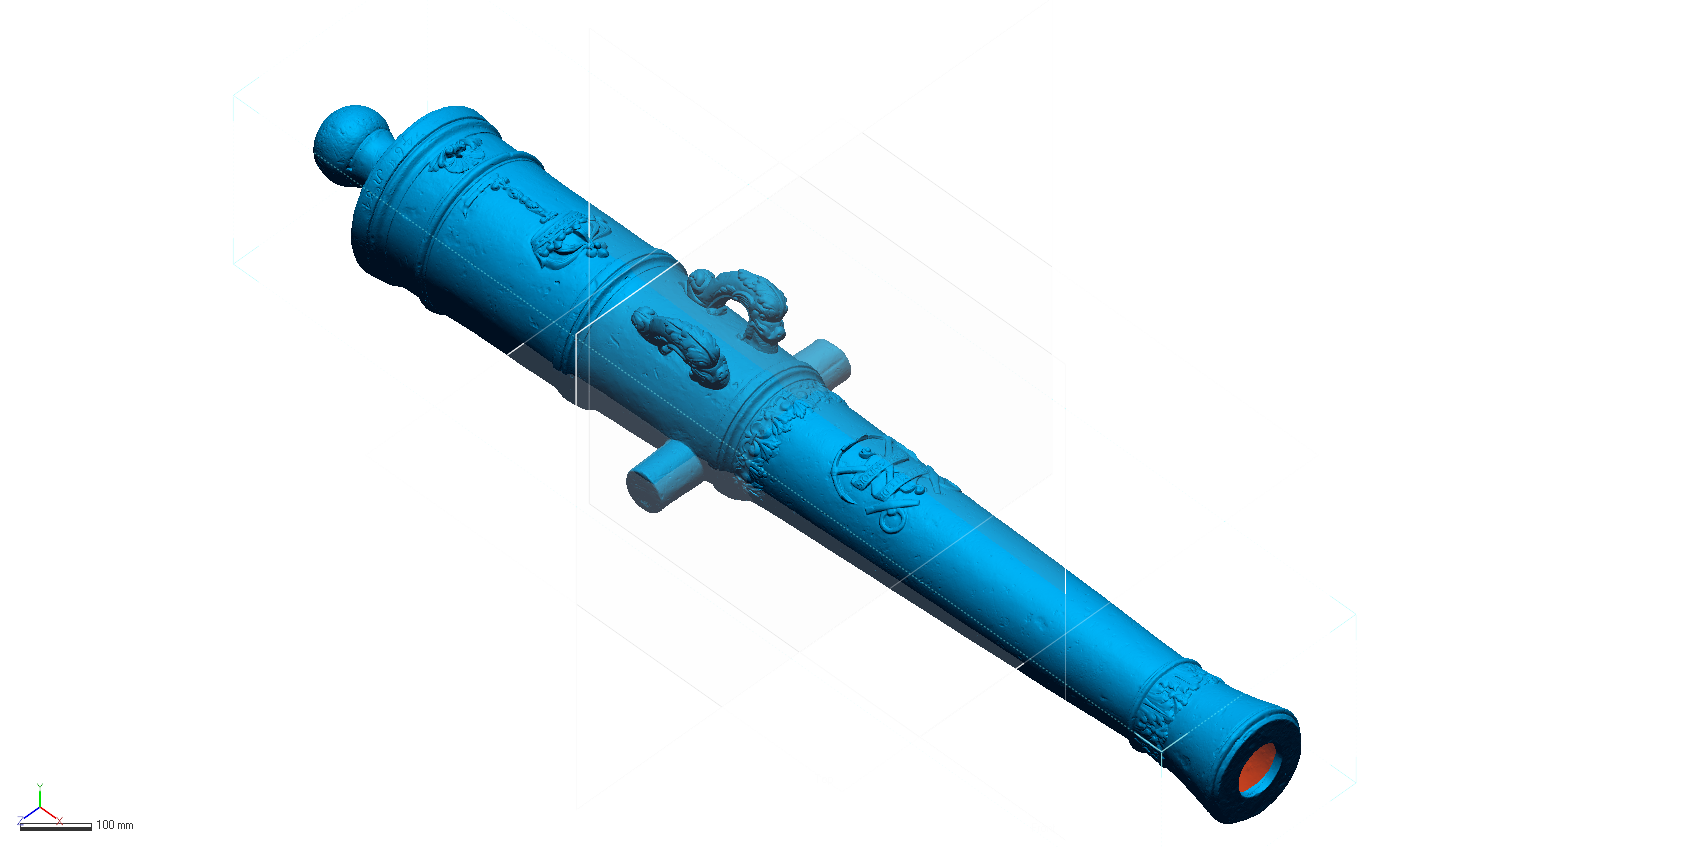
\includegraphics[width=\linewidth]{FigLSC2}
\caption{Three-dimensional mesh used to generate the freeform CAD model. Also see the Supplementary 3D model to interact with the 3D mesh for the cannon.}
\label{fig:Fig2}
\end{figure}

A custom patch network was designed to capture the vagaries of the mesh in a surface model. Three-dimensional contour curves were applied along high curvature areas of the mesh used as the basis for the initial layout of the patch network. The initial iteration of the patch network enlisted an auto estimation of the number of patches necessary, which was subsequently refined through a series of comparisons between the surface model and the mesh in Geomagic Control X.

Following design and layout of the initial patch network, each of the iteration was exported to Geomagic Control X to identify areas of the design that exceeded the specified tolerance and required revision (see Figure ~\ref{fig:Fig4}). Development of the final surface model was an iterative process that resulted in a total of five revisions to the initial design of the patch network, yielding a freeform surface model that meets with the tolerance (0.1 mm) specified for this project.

\begin{figure}[ht]\centering
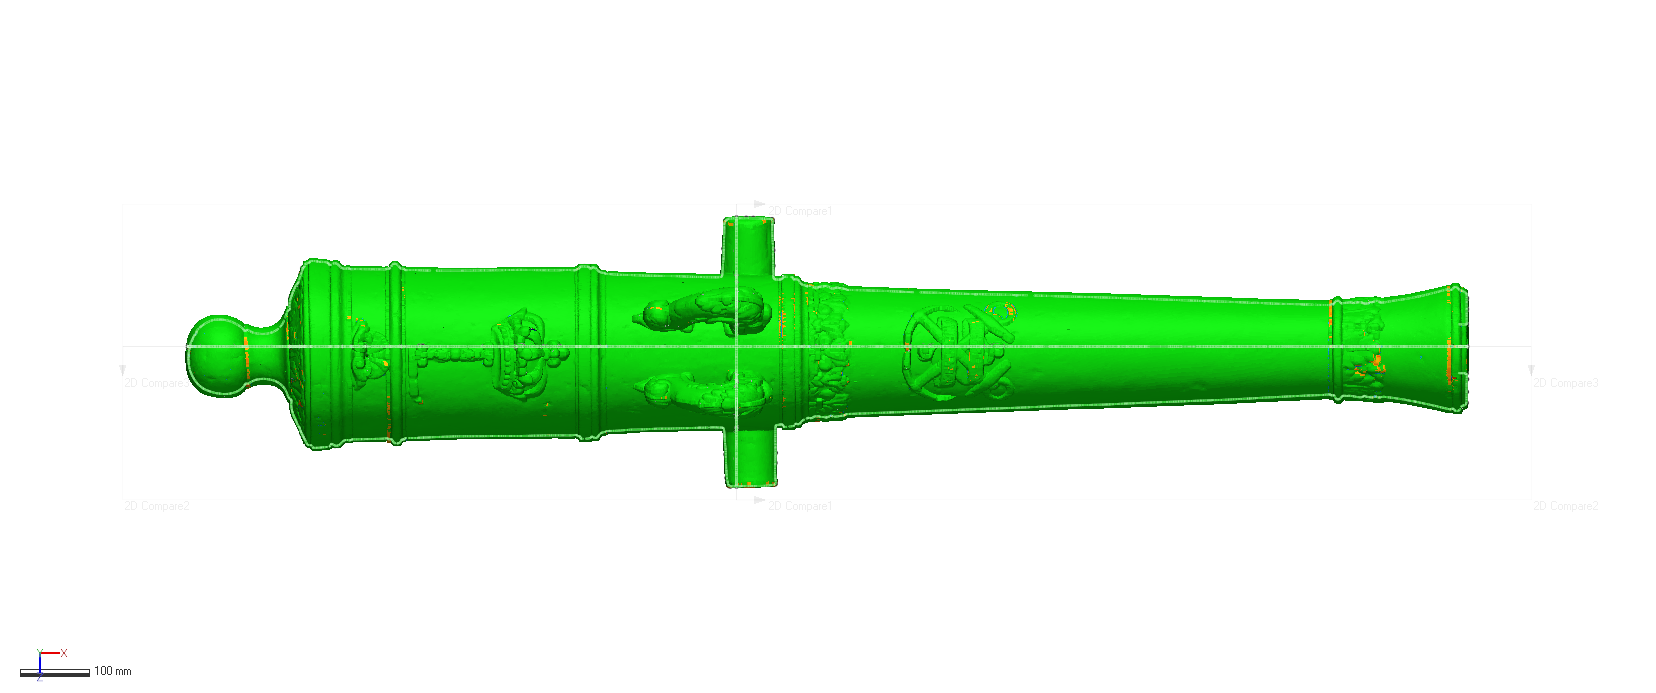
\includegraphics[width=\linewidth]{FigCanDev}
\caption{Third iteration of the custom patch network (freeform CAD model) in Geomagic Control X, illustrating the two cross sections, areas of the CAD model that were within the specified 0.1 mm tolerance (green), and areas of the patch network that warranted additional modeling (light blue and orange).}
\label{fig:Fig4}
\end{figure}

Revisions to the patch network were conducted by shuffling patch groups, editing, and inserting splines. Upon rendering the final surface model, it was exported as STEP and IGES files, then rendered in KeyShot. The integration of the cannon into an assembly (i.e., carriage, etc.) would warrant additional inspection, including 3D geometric dimensioning and tolerancing (3D GD\&T) \citep{RN5875,RN5874,RN5876}, to describe nominal geometry and the allowable variation prior to the manufacture of the cannon, and enlist computer aided manufacturing (CAM) for production \citep{RN5877,RN5878}.

\section*{Results and Discussion}

The iterative approach to modeling one of the bronze cannons from the La Belle excavations resulted in an accurate surface model of the cannon (Figure ~\ref{fig:Fig5}) that follows best practices, and complies with both the London Charter \citep{RN5872} and the Seville Principles \citep{RN5873}. The vent and bore of the cannon were sealed in the final surface model; however, those areas of the surface model can be removed, then extruded to render a parametric solid model prior to casting. The development of the 3D surface model greatly expedites that process, and provides an accurate model that is true to the original design, while also including specific, detailed attributes associated with its' wear, transport, and use-life.

\begin{figure}[ht]\centering
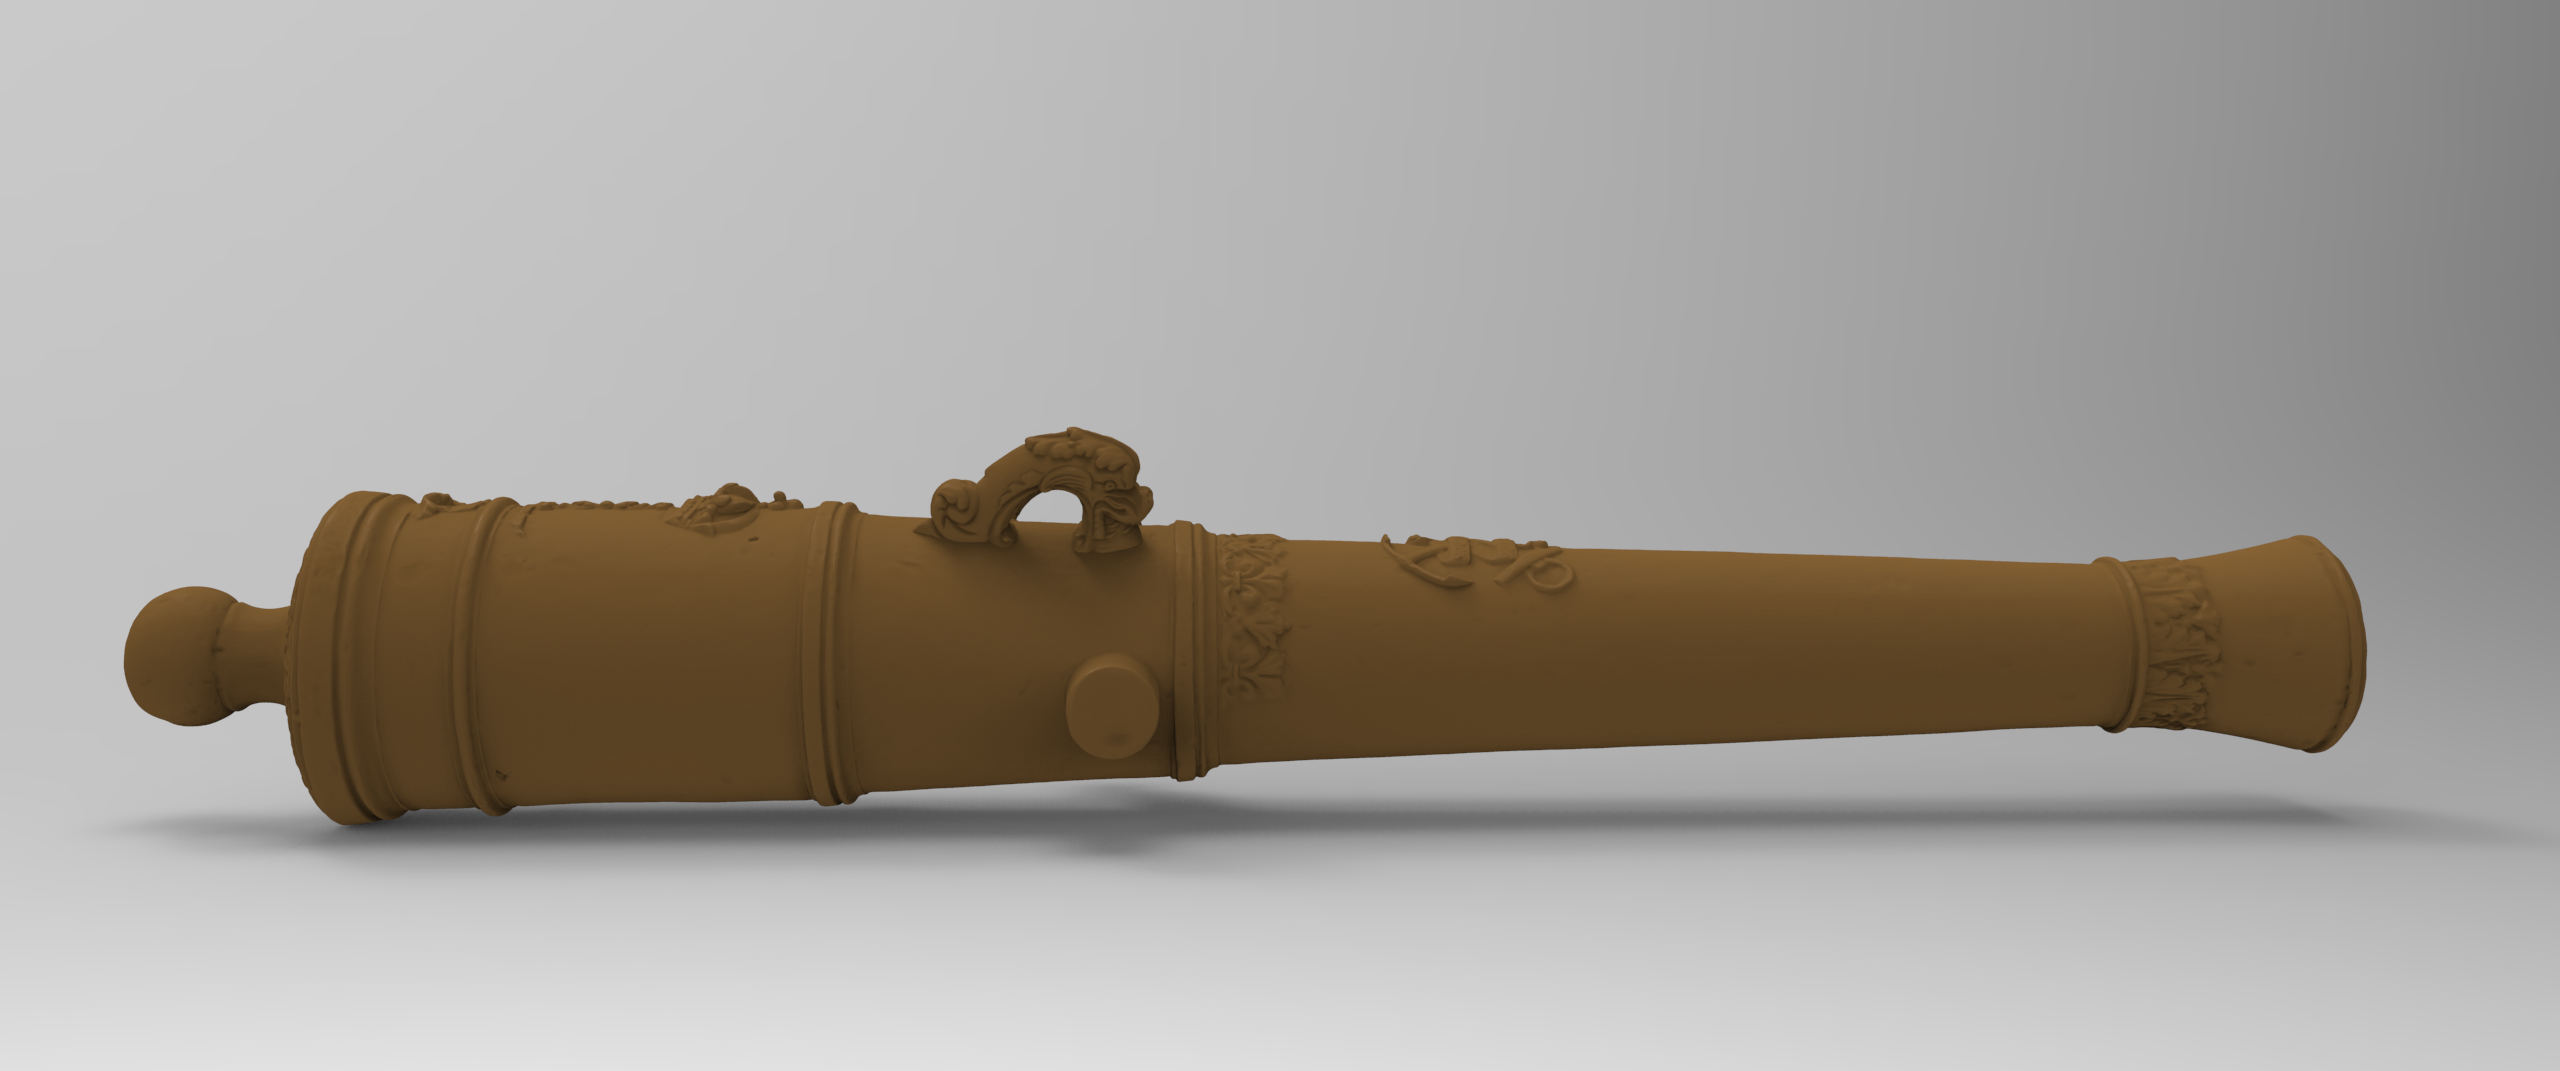
\includegraphics[width=\linewidth]{FigSurfaceModel}
\caption{Three-dimensional surface model for one of three bronze cannons recovered during the La Belle excavations.}
\label{fig:Fig5}
\end{figure}

Three-dimensional prints of the cannon (and the handles, separately) have been generated, and were recently used at the Technology in Archaeology Academy in Fredericksburg, Texas, organised by the Texas Archeological Society. The 3D prints of the cannon handles were scanned at the Academy with the same scanner used to scan the cannon (Creaform GoSCAN20), then compared with the final surface model of the handle generated by this project using a 0.3 mm tolerance (Figure ~\ref{fig:Fig6}). This exercise made us curious regarding the variable 3D printing resins (and printers), and which would provide the most accurate model. While that topic is not explored here, it does seem that future comparative analyses of 3D printers and the various resins that they can use would benefit discussions of 3D printing and additive manufacturing related to the reproduction archaeological artefacts.

\begin{figure}[ht]\centering
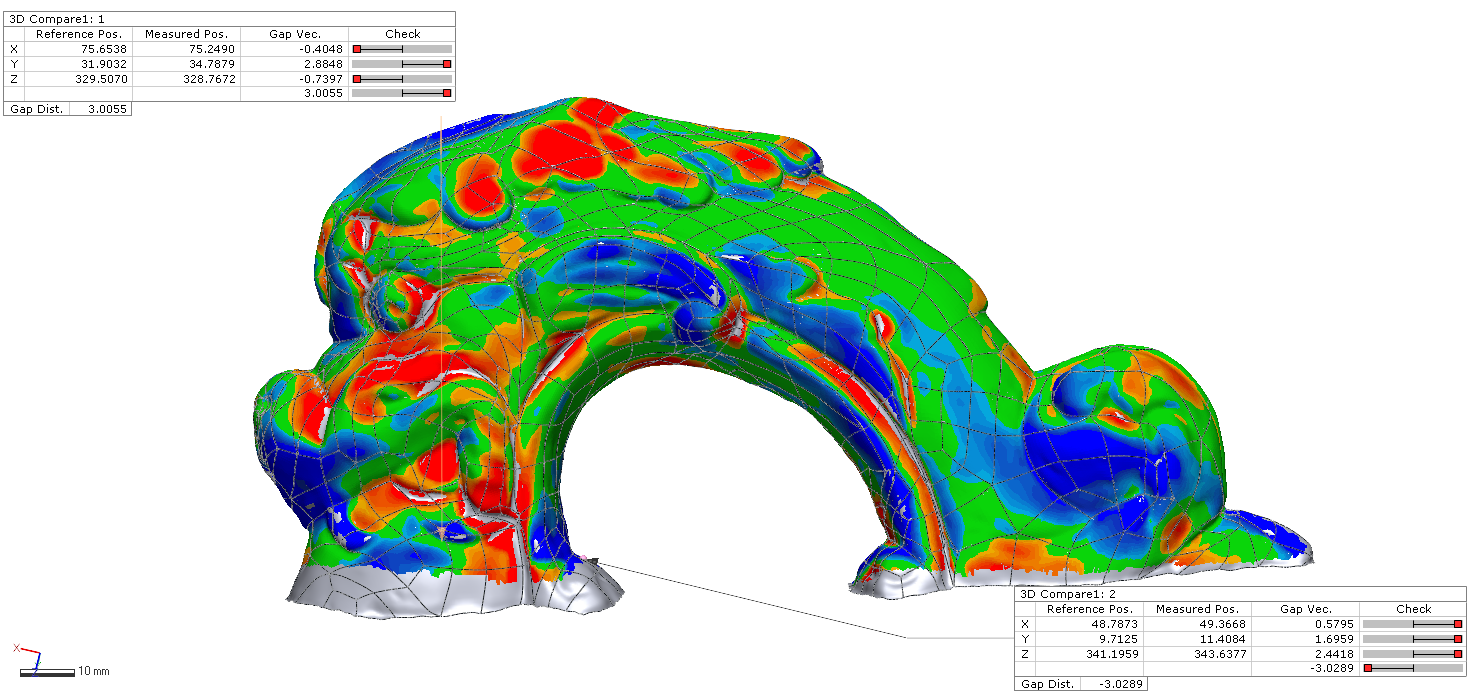
\includegraphics[width=\linewidth]{CannonCompare}
\caption{The 3D printed model of the cannon handle was scanned by workshop participants, then compared (0.3 mm tolerance) with the 3D surface model of the cannon. The two call-outs represent the maximum deviations of the 3D print above and below the surface model. Areas in green meet the specified tolerance, and areas above (red gradient) and below tolerance (blue gradient) are also noted.}
\label{fig:Fig6}
\end{figure}

Since completion of the conservation process, the exterior of the cannon has been slowly oxidising (tarnishing), a process that requires continual monitoring and spot treatments by curators, and is visible in the textured mesh. While not a formal goal established by or for this project, it may be possible to define how much of the cannon (volume and area) is currently tarnished by enlisting the texture data from the mesh. Our rationale is that a subsequent scan, collected---perhaps---in three to five years with the same equipment, has the potential to calculate and compare those areas that display oxidation. That information could then be used to calculate the rate of oxidation over the external surface, and develop a trajectory associated with the oxidation rate. The oxidation trajectory could then be used to identify a specific threshold at which point the cannon would warrant further conservation. This manner of qualitative and quantitative data could be used in a variety of funding proposals aimed at managing the advancement of oxidation along the cannon exterior. Demonstrating the rate of oxidation advancement could prove a useful metric for the continued management of the cannon, as well as other collections where active corrosion is an issue.

An additional observation resulting from the scanning process involves areas of presumed tool marks associated with the addition of decorative elements on the surface of the original mould model. Though speculative, examination of these areas using the 3D mesh and 3D surface model may assist in further developing hypotheses associated with the manufacturing process used to cast the cannon. At present, it is unclear whether these marks were left behind as a consequence of applying the decorative elements to the cannon model, as traces of tool marks on the moulds, or as a result of the finishing process after casting of the cannon was complete \cite[358]{RN5763}.

It is equally curious just how closely the single-use moulds assumed to have been used to manufacture these cannons actually align with one another. This research question could be tested through the collection of 3D scan data for the other two bronze cannons recovered from the La Belle, followed by a comparison of those meshes with the model generated through this endeavour. Using computer aided inspection, deviations could be calculated for the whole of the cannon as well as individual design elements, providing an improved comprehension of the process employed in the design, modeling, and casting by French metalsmiths.

\section*{Conclusion}

The mesh and freeform surface model generated by this project are useful in ways that reach beyond the scope of the initial undertaking. The surface model was created in following with best practices, resulting in the iterative development of a surface model that meets the specified 0.1 mm tolerance. While hopeful that the cannon will eventually be reproduced and displayed in the Musée National de la Marine in the Republic of France, there are a large number of ancillary analytical, educational, and interpretive pursuits that can leverage the surface model and the mesh in the interim.

\section*{Acknowledgments}

We extend our gratitude to the Bullock Texas State History Museum for access, and the Texas Historical Commission for the requisite permissions needed to scan the cannon. The cannon derives from the contents of \textit{La Belle}, all of which is the property of the Republic of France and from the collection of the Musée national de la Marine. Our thanks to Kersten Bergstrom, Tad Britt, and Bernard K. Means for their thoughtful comments on an earlier draft.

\section*{References}

\bibliographystyle{model6-num-names}
\bibliography{mybibfile}

\end{document}